\documentclass[twoside]{book}

% Packages required by doxygen
\usepackage{fixltx2e}
\usepackage{calc}
\usepackage{doxygen}
\usepackage[export]{adjustbox} % also loads graphicx
\usepackage{graphicx}
\usepackage[utf8]{inputenc}
\usepackage{makeidx}
\usepackage{multicol}
\usepackage{multirow}
\PassOptionsToPackage{warn}{textcomp}
\usepackage{textcomp}
\usepackage[nointegrals]{wasysym}
\usepackage[table]{xcolor}

% Font selection
\usepackage[T1]{fontenc}
\usepackage[scaled=.90]{helvet}
\usepackage{courier}
\usepackage{amssymb}
\usepackage{sectsty}
\renewcommand{\familydefault}{\sfdefault}
\allsectionsfont{%
  \fontseries{bc}\selectfont%
  \color{darkgray}%
}
\renewcommand{\DoxyLabelFont}{%
  \fontseries{bc}\selectfont%
  \color{darkgray}%
}
\newcommand{\+}{\discretionary{\mbox{\scriptsize$\hookleftarrow$}}{}{}}

% Page & text layout
\usepackage{geometry}
\geometry{%
  a4paper,%
  top=2.5cm,%
  bottom=2.5cm,%
  left=2.5cm,%
  right=2.5cm%
}
\tolerance=750
\hfuzz=15pt
\hbadness=750
\setlength{\emergencystretch}{15pt}
\setlength{\parindent}{0cm}
\setlength{\parskip}{3ex plus 2ex minus 2ex}
\makeatletter
\renewcommand{\paragraph}{%
  \@startsection{paragraph}{4}{0ex}{-1.0ex}{1.0ex}{%
    \normalfont\normalsize\bfseries\SS@parafont%
  }%
}
\renewcommand{\subparagraph}{%
  \@startsection{subparagraph}{5}{0ex}{-1.0ex}{1.0ex}{%
    \normalfont\normalsize\bfseries\SS@subparafont%
  }%
}
\makeatother

% Headers & footers
\usepackage{fancyhdr}
\pagestyle{fancyplain}
\fancyhead[LE]{\fancyplain{}{\bfseries\thepage}}
\fancyhead[CE]{\fancyplain{}{}}
\fancyhead[RE]{\fancyplain{}{\bfseries\leftmark}}
\fancyhead[LO]{\fancyplain{}{\bfseries\rightmark}}
\fancyhead[CO]{\fancyplain{}{}}
\fancyhead[RO]{\fancyplain{}{\bfseries\thepage}}
\fancyfoot[LE]{\fancyplain{}{}}
\fancyfoot[CE]{\fancyplain{}{}}
\fancyfoot[RE]{\fancyplain{}{\bfseries\scriptsize Generated by Doxygen }}
\fancyfoot[LO]{\fancyplain{}{\bfseries\scriptsize Generated by Doxygen }}
\fancyfoot[CO]{\fancyplain{}{}}
\fancyfoot[RO]{\fancyplain{}{}}
\renewcommand{\footrulewidth}{0.4pt}
\renewcommand{\chaptermark}[1]{%
  \markboth{#1}{}%
}
\renewcommand{\sectionmark}[1]{%
  \markright{\thesection\ #1}%
}

% Indices & bibliography
\usepackage{natbib}
\usepackage[titles]{tocloft}
\setcounter{tocdepth}{3}
\setcounter{secnumdepth}{5}
\makeindex

% Hyperlinks (required, but should be loaded last)
\usepackage{ifpdf}
\ifpdf
  \usepackage[pdftex,pagebackref=true]{hyperref}
\else
  \usepackage[ps2pdf,pagebackref=true]{hyperref}
\fi
\hypersetup{%
  colorlinks=true,%
  linkcolor=blue,%
  citecolor=blue,%
  unicode%
}

% Custom commands
\newcommand{\clearemptydoublepage}{%
  \newpage{\pagestyle{empty}\cleardoublepage}%
}

\usepackage{caption}
\captionsetup{labelsep=space,justification=centering,font={bf},singlelinecheck=off,skip=4pt,position=top}

%===== C O N T E N T S =====

\begin{document}

% Titlepage & ToC
\hypersetup{pageanchor=false,
             bookmarksnumbered=true,
             pdfencoding=unicode
            }
\pagenumbering{roman}
\begin{titlepage}
\vspace*{7cm}
\begin{center}%
{\Large My Project }\\
\vspace*{1cm}
{\large Generated by Doxygen 1.8.11}\\
\end{center}
\end{titlepage}
\clearemptydoublepage
\tableofcontents
\clearemptydoublepage
\pagenumbering{arabic}
\hypersetup{pageanchor=true}

%--- Begin generated contents ---
\chapter{Namespace Index}
\section{Packages}
Here are the packages with brief descriptions (if available)\+:\begin{DoxyCompactList}
\item\contentsline{section}{\hyperlink{namespace_plex_byte}{Plex\+Byte} }{\pageref{namespace_plex_byte}}{}
\item\contentsline{section}{\hyperlink{namespace_plex_byte_1_1_mo_cap}{Plex\+Byte.\+Mo\+Cap} }{\pageref{namespace_plex_byte_1_1_mo_cap}}{}
\item\contentsline{section}{\hyperlink{namespace_plex_byte_1_1_mo_cap_1_1_backend}{Plex\+Byte.\+Mo\+Cap.\+Backend} }{\pageref{namespace_plex_byte_1_1_mo_cap_1_1_backend}}{}
\end{DoxyCompactList}

\chapter{Hierarchical Index}
\section{Class Hierarchy}
This inheritance list is sorted roughly, but not completely, alphabetically\+:\begin{DoxyCompactList}
\item I\+Disposable\begin{DoxyCompactList}
\item \contentsline{section}{Plex\+Byte.\+Mo\+Cap.\+Backend.\+Backend\+Service}{\pageref{class_plex_byte_1_1_mo_cap_1_1_backend_1_1_backend_service}}{}
\end{DoxyCompactList}
\end{DoxyCompactList}

\chapter{Class Index}
\section{Class List}
Here are the classes, structs, unions and interfaces with brief descriptions\+:\begin{DoxyCompactList}
\item\contentsline{section}{\hyperlink{class_plex_byte_1_1_mo_cap_1_1_interactions_1_1_account}{Plex\+Byte.\+Mo\+Cap.\+Interactions.\+Account} }{\pageref{class_plex_byte_1_1_mo_cap_1_1_interactions_1_1_account}}{}
\item\contentsline{section}{\hyperlink{class_plex_byte_1_1_mo_cap_1_1_interactions_1_1_expense}{Plex\+Byte.\+Mo\+Cap.\+Interactions.\+Expense} }{\pageref{class_plex_byte_1_1_mo_cap_1_1_interactions_1_1_expense}}{}
\item\contentsline{section}{\hyperlink{interface_plex_byte_1_1_mo_cap_1_1_interactions_1_1_i_account}{Plex\+Byte.\+Mo\+Cap.\+Interactions.\+I\+Account} }{\pageref{interface_plex_byte_1_1_mo_cap_1_1_interactions_1_1_i_account}}{}
\item\contentsline{section}{\hyperlink{interface_plex_byte_1_1_mo_cap_1_1_interactions_1_1_i_expense}{Plex\+Byte.\+Mo\+Cap.\+Interactions.\+I\+Expense} }{\pageref{interface_plex_byte_1_1_mo_cap_1_1_interactions_1_1_i_expense}}{}
\item\contentsline{section}{\hyperlink{interface_plex_byte_1_1_mo_cap_1_1_interactions_1_1_i_interaction}{Plex\+Byte.\+Mo\+Cap.\+Interactions.\+I\+Interaction} }{\pageref{interface_plex_byte_1_1_mo_cap_1_1_interactions_1_1_i_interaction}}{}
\item\contentsline{section}{\hyperlink{interface_plex_byte_1_1_mo_cap_1_1_interactions_1_1_i_interaction_factory}{Plex\+Byte.\+Mo\+Cap.\+Interactions.\+I\+Interaction\+Factory} }{\pageref{interface_plex_byte_1_1_mo_cap_1_1_interactions_1_1_i_interaction_factory}}{}
\item\contentsline{section}{\hyperlink{class_plex_byte_1_1_mo_cap_1_1_interactions_1_1_interaction}{Plex\+Byte.\+Mo\+Cap.\+Interactions.\+Interaction} }{\pageref{class_plex_byte_1_1_mo_cap_1_1_interactions_1_1_interaction}}{}
\item\contentsline{section}{\hyperlink{class_plex_byte_1_1_mo_cap_1_1_interactions_1_1_interaction_event_args}{Plex\+Byte.\+Mo\+Cap.\+Interactions.\+Interaction\+Event\+Args} }{\pageref{class_plex_byte_1_1_mo_cap_1_1_interactions_1_1_interaction_event_args}}{}
\item\contentsline{section}{\hyperlink{class_plex_byte_1_1_mo_cap_1_1_interactions_1_1_interaction_factory}{Plex\+Byte.\+Mo\+Cap.\+Interactions.\+Interaction\+Factory} }{\pageref{class_plex_byte_1_1_mo_cap_1_1_interactions_1_1_interaction_factory}}{}
\item\contentsline{section}{\hyperlink{interface_plex_byte_1_1_mo_cap_1_1_interactions_1_1_i_object_factory}{Plex\+Byte.\+Mo\+Cap.\+Interactions.\+I\+Object\+Factory} }{\pageref{interface_plex_byte_1_1_mo_cap_1_1_interactions_1_1_i_object_factory}}{}
\item\contentsline{section}{\hyperlink{interface_plex_byte_1_1_mo_cap_1_1_interactions_1_1_i_project}{Plex\+Byte.\+Mo\+Cap.\+Interactions.\+I\+Project} }{\pageref{interface_plex_byte_1_1_mo_cap_1_1_interactions_1_1_i_project}}{}
\item\contentsline{section}{\hyperlink{interface_plex_byte_1_1_mo_cap_1_1_interactions_1_1_i_survey}{Plex\+Byte.\+Mo\+Cap.\+Interactions.\+I\+Survey} }{\pageref{interface_plex_byte_1_1_mo_cap_1_1_interactions_1_1_i_survey}}{}
\item\contentsline{section}{\hyperlink{interface_plex_byte_1_1_mo_cap_1_1_interactions_1_1_i_survey_option}{Plex\+Byte.\+Mo\+Cap.\+Interactions.\+I\+Survey\+Option} \\*The survey option interface }{\pageref{interface_plex_byte_1_1_mo_cap_1_1_interactions_1_1_i_survey_option}}{}
\item\contentsline{section}{\hyperlink{interface_plex_byte_1_1_mo_cap_1_1_interactions_1_1_i_task}{Plex\+Byte.\+Mo\+Cap.\+Interactions.\+I\+Task} }{\pageref{interface_plex_byte_1_1_mo_cap_1_1_interactions_1_1_i_task}}{}
\item\contentsline{section}{\hyperlink{interface_plex_byte_1_1_mo_cap_1_1_interactions_1_1_i_timeslice}{Plex\+Byte.\+Mo\+Cap.\+Interactions.\+I\+Timeslice} }{\pageref{interface_plex_byte_1_1_mo_cap_1_1_interactions_1_1_i_timeslice}}{}
\item\contentsline{section}{\hyperlink{interface_plex_byte_1_1_mo_cap_1_1_interactions_1_1_i_vote}{Plex\+Byte.\+Mo\+Cap.\+Interactions.\+I\+Vote} \\*The vote interface }{\pageref{interface_plex_byte_1_1_mo_cap_1_1_interactions_1_1_i_vote}}{}
\item\contentsline{section}{\hyperlink{class_plex_byte_1_1_mo_cap_1_1_interactions_1_1_object_factory}{Plex\+Byte.\+Mo\+Cap.\+Interactions.\+Object\+Factory} }{\pageref{class_plex_byte_1_1_mo_cap_1_1_interactions_1_1_object_factory}}{}
\item\contentsline{section}{\hyperlink{class_plex_byte_1_1_mo_cap_1_1_interactions_1_1_project}{Plex\+Byte.\+Mo\+Cap.\+Interactions.\+Project} }{\pageref{class_plex_byte_1_1_mo_cap_1_1_interactions_1_1_project}}{}
\item\contentsline{section}{\hyperlink{class_plex_byte_1_1_mo_cap_1_1_interactions_1_1_survey}{Plex\+Byte.\+Mo\+Cap.\+Interactions.\+Survey} }{\pageref{class_plex_byte_1_1_mo_cap_1_1_interactions_1_1_survey}}{}
\item\contentsline{section}{\hyperlink{class_plex_byte_1_1_mo_cap_1_1_interactions_1_1_survey_option}{Plex\+Byte.\+Mo\+Cap.\+Interactions.\+Survey\+Option} \\*The survey option class, which hold the option text }{\pageref{class_plex_byte_1_1_mo_cap_1_1_interactions_1_1_survey_option}}{}
\item\contentsline{section}{\hyperlink{class_plex_byte_1_1_mo_cap_1_1_interactions_1_1_task}{Plex\+Byte.\+Mo\+Cap.\+Interactions.\+Task} }{\pageref{class_plex_byte_1_1_mo_cap_1_1_interactions_1_1_task}}{}
\item\contentsline{section}{\hyperlink{class_plex_byte_1_1_mo_cap_1_1_interactions_1_1_timeslice}{Plex\+Byte.\+Mo\+Cap.\+Interactions.\+Timeslice} }{\pageref{class_plex_byte_1_1_mo_cap_1_1_interactions_1_1_timeslice}}{}
\item\contentsline{section}{\hyperlink{class_plex_byte_1_1_mo_cap_1_1_interactions_1_1_vote}{Plex\+Byte.\+Mo\+Cap.\+Interactions.\+Vote} \\*This class holds information about a users choice, containing the user and his choice selected }{\pageref{class_plex_byte_1_1_mo_cap_1_1_interactions_1_1_vote}}{}
\end{DoxyCompactList}

\chapter{File Index}
\section{File List}
Here is a list of all files with brief descriptions\+:\begin{DoxyCompactList}
\item\contentsline{section}{D\+:/\+Users/\+Christian\+B/\+Documents/\+\_\+\+H\+F Infomatik/\+Git\+Hub\+\_\+\+Repos/\+Mo\+Cap/\+Plex\+Byte.\+Mo\+Cap/\+Plex\+Byte.\+Mo\+Cap.\+Backend/\hyperlink{_backend_service_8cs}{Backend\+Service.\+cs} }{\pageref{_backend_service_8cs}}{}
\end{DoxyCompactList}

\chapter{Namespace Documentation}
\hypertarget{namespace_plex_byte}{}\section{Plex\+Byte Namespace Reference}
\label{namespace_plex_byte}\index{Plex\+Byte@{Plex\+Byte}}
\subsection*{Namespaces}
\begin{DoxyCompactItemize}
\item 
namespace \hyperlink{namespace_plex_byte_1_1_mo_cap}{Mo\+Cap}
\end{DoxyCompactItemize}

\hypertarget{namespace_plex_byte_1_1_mo_cap}{}\section{Plex\+Byte.\+Mo\+Cap Namespace Reference}
\label{namespace_plex_byte_1_1_mo_cap}\index{Plex\+Byte.\+Mo\+Cap@{Plex\+Byte.\+Mo\+Cap}}
\subsection*{Namespaces}
\begin{DoxyCompactItemize}
\item 
namespace \hyperlink{namespace_plex_byte_1_1_mo_cap_1_1_win_forms}{Win\+Forms}
\end{DoxyCompactItemize}

\hypertarget{namespace_plex_byte_1_1_mo_cap_1_1_win_forms}{}\section{Plex\+Byte.\+Mo\+Cap.\+Win\+Forms Namespace Reference}
\label{namespace_plex_byte_1_1_mo_cap_1_1_win_forms}\index{Plex\+Byte.\+Mo\+Cap.\+Win\+Forms@{Plex\+Byte.\+Mo\+Cap.\+Win\+Forms}}
\subsection*{Classes}
\begin{DoxyCompactItemize}
\item 
class \hyperlink{class_plex_byte_1_1_mo_cap_1_1_win_forms_1_1frm___mo_cap_main}{frm\+\_\+\+Mo\+Cap\+Main}
\item 
class \hyperlink{class_plex_byte_1_1_mo_cap_1_1_win_forms_1_1frm___test}{frm\+\_\+\+Test}
\item 
class {\bfseries Program}
\end{DoxyCompactItemize}

\chapter{Class Documentation}
\hypertarget{class_plex_byte_1_1_mo_cap_1_1_win_forms_1_1frm___mo_cap_main}{}\section{Plex\+Byte.\+Mo\+Cap.\+Win\+Forms.\+frm\+\_\+\+Mo\+Cap\+Main Class Reference}
\label{class_plex_byte_1_1_mo_cap_1_1_win_forms_1_1frm___mo_cap_main}\index{Plex\+Byte.\+Mo\+Cap.\+Win\+Forms.\+frm\+\_\+\+Mo\+Cap\+Main@{Plex\+Byte.\+Mo\+Cap.\+Win\+Forms.\+frm\+\_\+\+Mo\+Cap\+Main}}
Inheritance diagram for Plex\+Byte.\+Mo\+Cap.\+Win\+Forms.\+frm\+\_\+\+Mo\+Cap\+Main\+:\begin{figure}[H]
\begin{center}
\leavevmode
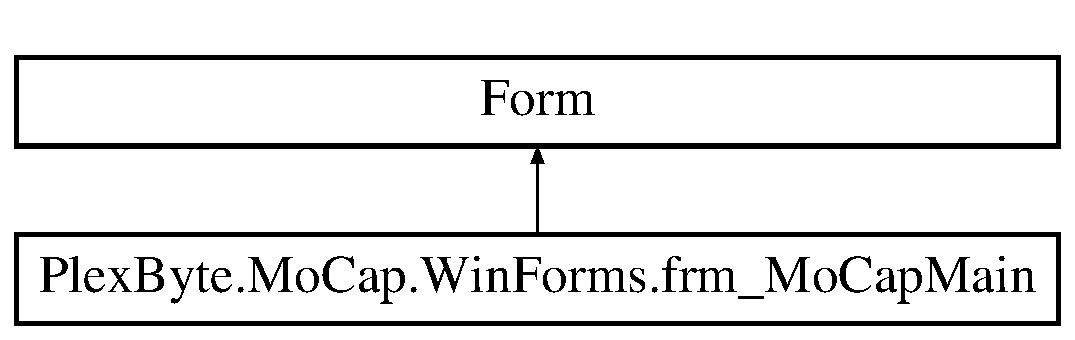
\includegraphics[height=2.000000cm]{class_plex_byte_1_1_mo_cap_1_1_win_forms_1_1frm___mo_cap_main}
\end{center}
\end{figure}
\subsection*{Public Member Functions}
\begin{DoxyCompactItemize}
\item 
\hyperlink{class_plex_byte_1_1_mo_cap_1_1_win_forms_1_1frm___mo_cap_main_ad5e74126f5d02438095f3cccee647767}{frm\+\_\+\+Mo\+Cap\+Main} ()
\item 
void \hyperlink{class_plex_byte_1_1_mo_cap_1_1_win_forms_1_1frm___mo_cap_main_a53f66c824f18a754a20bfee1ef13873e}{Show\+Error\+Message} (string p\+Error\+Message)
\end{DoxyCompactItemize}
\subsection*{Public Attributes}
\begin{DoxyCompactItemize}
\item 
Dock\+Panel \hyperlink{class_plex_byte_1_1_mo_cap_1_1_win_forms_1_1frm___mo_cap_main_a523b01d4a9ec5573c7e42b439644c9ee}{Panel} =$>$ dock\+Panel1
\item 
U\+I\+Manager \hyperlink{class_plex_byte_1_1_mo_cap_1_1_win_forms_1_1frm___mo_cap_main_a33aa80ec18c499177631895f86eec5ba}{U\+I\+Manager} =$>$ \+\_\+ui\+Manager
\end{DoxyCompactItemize}
\subsection*{Protected Member Functions}
\begin{DoxyCompactItemize}
\item 
override void \hyperlink{class_plex_byte_1_1_mo_cap_1_1_win_forms_1_1frm___mo_cap_main_a3e2826ccdbfc7be1865c079bf9b4c5a6}{Dispose} (bool disposing)
\begin{DoxyCompactList}\small\item\em Clean up any resources being used. \end{DoxyCompactList}\end{DoxyCompactItemize}


\subsection{Detailed Description}


Definition at line 13 of file frm\+\_\+\+Mo\+Cap\+Main.\+cs.



\subsection{Constructor \& Destructor Documentation}
\index{Plex\+Byte\+::\+Mo\+Cap\+::\+Win\+Forms\+::frm\+\_\+\+Mo\+Cap\+Main@{Plex\+Byte\+::\+Mo\+Cap\+::\+Win\+Forms\+::frm\+\_\+\+Mo\+Cap\+Main}!frm\+\_\+\+Mo\+Cap\+Main@{frm\+\_\+\+Mo\+Cap\+Main}}
\index{frm\+\_\+\+Mo\+Cap\+Main@{frm\+\_\+\+Mo\+Cap\+Main}!Plex\+Byte\+::\+Mo\+Cap\+::\+Win\+Forms\+::frm\+\_\+\+Mo\+Cap\+Main@{Plex\+Byte\+::\+Mo\+Cap\+::\+Win\+Forms\+::frm\+\_\+\+Mo\+Cap\+Main}}
\subsubsection[{\texorpdfstring{frm\+\_\+\+Mo\+Cap\+Main()}{frm_MoCapMain()}}]{\setlength{\rightskip}{0pt plus 5cm}Plex\+Byte.\+Mo\+Cap.\+Win\+Forms.\+frm\+\_\+\+Mo\+Cap\+Main.\+frm\+\_\+\+Mo\+Cap\+Main (
\begin{DoxyParamCaption}
{}
\end{DoxyParamCaption}
)}\hypertarget{class_plex_byte_1_1_mo_cap_1_1_win_forms_1_1frm___mo_cap_main_ad5e74126f5d02438095f3cccee647767}{}\label{class_plex_byte_1_1_mo_cap_1_1_win_forms_1_1frm___mo_cap_main_ad5e74126f5d02438095f3cccee647767}


Definition at line 20 of file frm\+\_\+\+Mo\+Cap\+Main.\+cs.



\subsection{Member Function Documentation}
\index{Plex\+Byte\+::\+Mo\+Cap\+::\+Win\+Forms\+::frm\+\_\+\+Mo\+Cap\+Main@{Plex\+Byte\+::\+Mo\+Cap\+::\+Win\+Forms\+::frm\+\_\+\+Mo\+Cap\+Main}!Dispose@{Dispose}}
\index{Dispose@{Dispose}!Plex\+Byte\+::\+Mo\+Cap\+::\+Win\+Forms\+::frm\+\_\+\+Mo\+Cap\+Main@{Plex\+Byte\+::\+Mo\+Cap\+::\+Win\+Forms\+::frm\+\_\+\+Mo\+Cap\+Main}}
\subsubsection[{\texorpdfstring{Dispose(bool disposing)}{Dispose(bool disposing)}}]{\setlength{\rightskip}{0pt plus 5cm}override void Plex\+Byte.\+Mo\+Cap.\+Win\+Forms.\+frm\+\_\+\+Mo\+Cap\+Main.\+Dispose (
\begin{DoxyParamCaption}
\item[{bool}]{disposing}
\end{DoxyParamCaption}
)\hspace{0.3cm}{\ttfamily [protected]}}\hypertarget{class_plex_byte_1_1_mo_cap_1_1_win_forms_1_1frm___mo_cap_main_a3e2826ccdbfc7be1865c079bf9b4c5a6}{}\label{class_plex_byte_1_1_mo_cap_1_1_win_forms_1_1frm___mo_cap_main_a3e2826ccdbfc7be1865c079bf9b4c5a6}


Clean up any resources being used. 


\begin{DoxyParams}{Parameters}
{\em disposing} & true if managed resources should be disposed; otherwise, false.\\
\hline
\end{DoxyParams}


Definition at line 14 of file frm\+\_\+\+Mo\+Cap\+Main.\+Designer.\+cs.

\index{Plex\+Byte\+::\+Mo\+Cap\+::\+Win\+Forms\+::frm\+\_\+\+Mo\+Cap\+Main@{Plex\+Byte\+::\+Mo\+Cap\+::\+Win\+Forms\+::frm\+\_\+\+Mo\+Cap\+Main}!Show\+Error\+Message@{Show\+Error\+Message}}
\index{Show\+Error\+Message@{Show\+Error\+Message}!Plex\+Byte\+::\+Mo\+Cap\+::\+Win\+Forms\+::frm\+\_\+\+Mo\+Cap\+Main@{Plex\+Byte\+::\+Mo\+Cap\+::\+Win\+Forms\+::frm\+\_\+\+Mo\+Cap\+Main}}
\subsubsection[{\texorpdfstring{Show\+Error\+Message(string p\+Error\+Message)}{ShowErrorMessage(string pErrorMessage)}}]{\setlength{\rightskip}{0pt plus 5cm}void Plex\+Byte.\+Mo\+Cap.\+Win\+Forms.\+frm\+\_\+\+Mo\+Cap\+Main.\+Show\+Error\+Message (
\begin{DoxyParamCaption}
\item[{string}]{p\+Error\+Message}
\end{DoxyParamCaption}
)}\hypertarget{class_plex_byte_1_1_mo_cap_1_1_win_forms_1_1frm___mo_cap_main_a53f66c824f18a754a20bfee1ef13873e}{}\label{class_plex_byte_1_1_mo_cap_1_1_win_forms_1_1frm___mo_cap_main_a53f66c824f18a754a20bfee1ef13873e}


Definition at line 39 of file frm\+\_\+\+Mo\+Cap\+Main.\+cs.



\subsection{Member Data Documentation}
\index{Plex\+Byte\+::\+Mo\+Cap\+::\+Win\+Forms\+::frm\+\_\+\+Mo\+Cap\+Main@{Plex\+Byte\+::\+Mo\+Cap\+::\+Win\+Forms\+::frm\+\_\+\+Mo\+Cap\+Main}!Panel@{Panel}}
\index{Panel@{Panel}!Plex\+Byte\+::\+Mo\+Cap\+::\+Win\+Forms\+::frm\+\_\+\+Mo\+Cap\+Main@{Plex\+Byte\+::\+Mo\+Cap\+::\+Win\+Forms\+::frm\+\_\+\+Mo\+Cap\+Main}}
\subsubsection[{\texorpdfstring{Panel}{Panel}}]{\setlength{\rightskip}{0pt plus 5cm}Dock\+Panel Plex\+Byte.\+Mo\+Cap.\+Win\+Forms.\+frm\+\_\+\+Mo\+Cap\+Main.\+Panel =$>$ dock\+Panel1}\hypertarget{class_plex_byte_1_1_mo_cap_1_1_win_forms_1_1frm___mo_cap_main_a523b01d4a9ec5573c7e42b439644c9ee}{}\label{class_plex_byte_1_1_mo_cap_1_1_win_forms_1_1frm___mo_cap_main_a523b01d4a9ec5573c7e42b439644c9ee}


Definition at line 15 of file frm\+\_\+\+Mo\+Cap\+Main.\+cs.

\index{Plex\+Byte\+::\+Mo\+Cap\+::\+Win\+Forms\+::frm\+\_\+\+Mo\+Cap\+Main@{Plex\+Byte\+::\+Mo\+Cap\+::\+Win\+Forms\+::frm\+\_\+\+Mo\+Cap\+Main}!U\+I\+Manager@{U\+I\+Manager}}
\index{U\+I\+Manager@{U\+I\+Manager}!Plex\+Byte\+::\+Mo\+Cap\+::\+Win\+Forms\+::frm\+\_\+\+Mo\+Cap\+Main@{Plex\+Byte\+::\+Mo\+Cap\+::\+Win\+Forms\+::frm\+\_\+\+Mo\+Cap\+Main}}
\subsubsection[{\texorpdfstring{U\+I\+Manager}{UIManager}}]{\setlength{\rightskip}{0pt plus 5cm}U\+I\+Manager Plex\+Byte.\+Mo\+Cap.\+Win\+Forms.\+frm\+\_\+\+Mo\+Cap\+Main.\+U\+I\+Manager =$>$ \+\_\+ui\+Manager}\hypertarget{class_plex_byte_1_1_mo_cap_1_1_win_forms_1_1frm___mo_cap_main_a33aa80ec18c499177631895f86eec5ba}{}\label{class_plex_byte_1_1_mo_cap_1_1_win_forms_1_1frm___mo_cap_main_a33aa80ec18c499177631895f86eec5ba}


Definition at line 16 of file frm\+\_\+\+Mo\+Cap\+Main.\+cs.



The documentation for this class was generated from the following files\+:\begin{DoxyCompactItemize}
\item 
D\+:/\+Users/\+Christian\+B/\+Documents/\+\_\+\+H\+F Infomatik/\+Git\+Hub\+\_\+\+Repos/\+Mo\+Cap/\+Plex\+Byte.\+Mo\+Cap/\+Plex\+Byte.\+Mo\+Cap.\+Win\+Forms/\hyperlink{frm___mo_cap_main_8cs}{frm\+\_\+\+Mo\+Cap\+Main.\+cs}\item 
D\+:/\+Users/\+Christian\+B/\+Documents/\+\_\+\+H\+F Infomatik/\+Git\+Hub\+\_\+\+Repos/\+Mo\+Cap/\+Plex\+Byte.\+Mo\+Cap/\+Plex\+Byte.\+Mo\+Cap.\+Win\+Forms/\hyperlink{frm___mo_cap_main_8_designer_8cs}{frm\+\_\+\+Mo\+Cap\+Main.\+Designer.\+cs}\end{DoxyCompactItemize}

\hypertarget{class_plex_byte_1_1_mo_cap_1_1_win_forms_1_1frm___test}{}\section{Plex\+Byte.\+Mo\+Cap.\+Win\+Forms.\+frm\+\_\+\+Test Class Reference}
\label{class_plex_byte_1_1_mo_cap_1_1_win_forms_1_1frm___test}\index{Plex\+Byte.\+Mo\+Cap.\+Win\+Forms.\+frm\+\_\+\+Test@{Plex\+Byte.\+Mo\+Cap.\+Win\+Forms.\+frm\+\_\+\+Test}}
Inheritance diagram for Plex\+Byte.\+Mo\+Cap.\+Win\+Forms.\+frm\+\_\+\+Test\+:\begin{figure}[H]
\begin{center}
\leavevmode
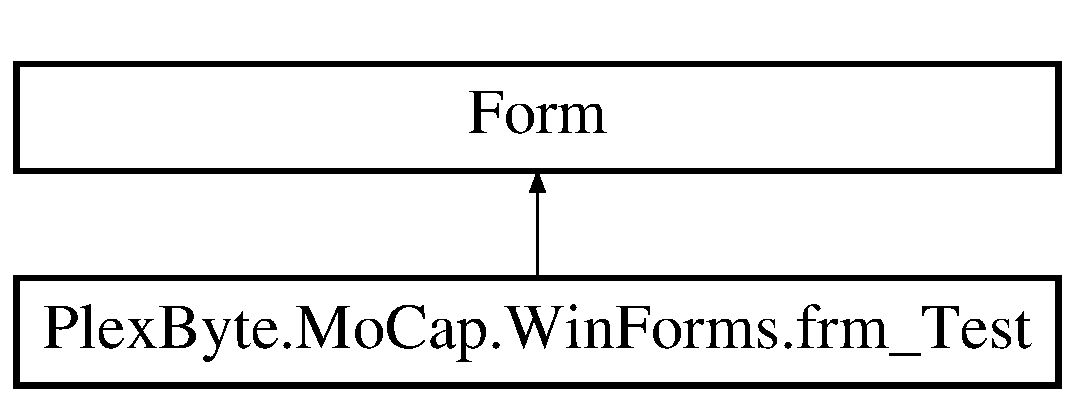
\includegraphics[height=2.000000cm]{class_plex_byte_1_1_mo_cap_1_1_win_forms_1_1frm___test}
\end{center}
\end{figure}
\subsection*{Public Member Functions}
\begin{DoxyCompactItemize}
\item 
\hyperlink{class_plex_byte_1_1_mo_cap_1_1_win_forms_1_1frm___test_abe776796af03a79e1064b4b557646a7b}{frm\+\_\+\+Test} ()
\end{DoxyCompactItemize}
\subsection*{Protected Member Functions}
\begin{DoxyCompactItemize}
\item 
override void \hyperlink{class_plex_byte_1_1_mo_cap_1_1_win_forms_1_1frm___test_a5c5e98552d5ddad39288d3ff784cd5f2}{Dispose} (bool disposing)
\begin{DoxyCompactList}\small\item\em Clean up any resources being used. \end{DoxyCompactList}\end{DoxyCompactItemize}


\subsection{Detailed Description}


Definition at line 6 of file frm\+\_\+\+Test.\+cs.



\subsection{Constructor \& Destructor Documentation}
\index{Plex\+Byte\+::\+Mo\+Cap\+::\+Win\+Forms\+::frm\+\_\+\+Test@{Plex\+Byte\+::\+Mo\+Cap\+::\+Win\+Forms\+::frm\+\_\+\+Test}!frm\+\_\+\+Test@{frm\+\_\+\+Test}}
\index{frm\+\_\+\+Test@{frm\+\_\+\+Test}!Plex\+Byte\+::\+Mo\+Cap\+::\+Win\+Forms\+::frm\+\_\+\+Test@{Plex\+Byte\+::\+Mo\+Cap\+::\+Win\+Forms\+::frm\+\_\+\+Test}}
\subsubsection[{\texorpdfstring{frm\+\_\+\+Test()}{frm_Test()}}]{\setlength{\rightskip}{0pt plus 5cm}Plex\+Byte.\+Mo\+Cap.\+Win\+Forms.\+frm\+\_\+\+Test.\+frm\+\_\+\+Test (
\begin{DoxyParamCaption}
{}
\end{DoxyParamCaption}
)}\hypertarget{class_plex_byte_1_1_mo_cap_1_1_win_forms_1_1frm___test_abe776796af03a79e1064b4b557646a7b}{}\label{class_plex_byte_1_1_mo_cap_1_1_win_forms_1_1frm___test_abe776796af03a79e1064b4b557646a7b}


Definition at line 8 of file frm\+\_\+\+Test.\+cs.



\subsection{Member Function Documentation}
\index{Plex\+Byte\+::\+Mo\+Cap\+::\+Win\+Forms\+::frm\+\_\+\+Test@{Plex\+Byte\+::\+Mo\+Cap\+::\+Win\+Forms\+::frm\+\_\+\+Test}!Dispose@{Dispose}}
\index{Dispose@{Dispose}!Plex\+Byte\+::\+Mo\+Cap\+::\+Win\+Forms\+::frm\+\_\+\+Test@{Plex\+Byte\+::\+Mo\+Cap\+::\+Win\+Forms\+::frm\+\_\+\+Test}}
\subsubsection[{\texorpdfstring{Dispose(bool disposing)}{Dispose(bool disposing)}}]{\setlength{\rightskip}{0pt plus 5cm}override void Plex\+Byte.\+Mo\+Cap.\+Win\+Forms.\+frm\+\_\+\+Test.\+Dispose (
\begin{DoxyParamCaption}
\item[{bool}]{disposing}
\end{DoxyParamCaption}
)\hspace{0.3cm}{\ttfamily [protected]}}\hypertarget{class_plex_byte_1_1_mo_cap_1_1_win_forms_1_1frm___test_a5c5e98552d5ddad39288d3ff784cd5f2}{}\label{class_plex_byte_1_1_mo_cap_1_1_win_forms_1_1frm___test_a5c5e98552d5ddad39288d3ff784cd5f2}


Clean up any resources being used. 


\begin{DoxyParams}{Parameters}
{\em disposing} & true if managed resources should be disposed; otherwise, false.\\
\hline
\end{DoxyParams}


Definition at line 14 of file frm\+\_\+\+Test.\+Designer.\+cs.



The documentation for this class was generated from the following files\+:\begin{DoxyCompactItemize}
\item 
D\+:/\+Users/\+Christian\+B/\+Documents/\+\_\+\+H\+F Infomatik/\+Git\+Hub\+\_\+\+Repos/\+Mo\+Cap/\+Plex\+Byte.\+Mo\+Cap/\+Plex\+Byte.\+Mo\+Cap.\+Win\+Forms/\hyperlink{frm___test_8cs}{frm\+\_\+\+Test.\+cs}\item 
D\+:/\+Users/\+Christian\+B/\+Documents/\+\_\+\+H\+F Infomatik/\+Git\+Hub\+\_\+\+Repos/\+Mo\+Cap/\+Plex\+Byte.\+Mo\+Cap/\+Plex\+Byte.\+Mo\+Cap.\+Win\+Forms/\hyperlink{frm___test_8_designer_8cs}{frm\+\_\+\+Test.\+Designer.\+cs}\end{DoxyCompactItemize}

\chapter{File Documentation}
\hypertarget{frm___mo_cap_main_8cs}{}\section{D\+:/\+Users/\+Christian\+B/\+Documents/\+\_\+\+HF Infomatik/\+Git\+Hub\+\_\+\+Repos/\+Mo\+Cap/\+Plex\+Byte.Mo\+Cap/\+Plex\+Byte.Mo\+Cap.\+Win\+Forms/frm\+\_\+\+Mo\+Cap\+Main.cs File Reference}
\label{frm___mo_cap_main_8cs}\index{D\+:/\+Users/\+Christian\+B/\+Documents/\+\_\+\+H\+F Infomatik/\+Git\+Hub\+\_\+\+Repos/\+Mo\+Cap/\+Plex\+Byte.\+Mo\+Cap/\+Plex\+Byte.\+Mo\+Cap.\+Win\+Forms/frm\+\_\+\+Mo\+Cap\+Main.\+cs@{D\+:/\+Users/\+Christian\+B/\+Documents/\+\_\+\+H\+F Infomatik/\+Git\+Hub\+\_\+\+Repos/\+Mo\+Cap/\+Plex\+Byte.\+Mo\+Cap/\+Plex\+Byte.\+Mo\+Cap.\+Win\+Forms/frm\+\_\+\+Mo\+Cap\+Main.\+cs}}
\subsection*{Classes}
\begin{DoxyCompactItemize}
\item 
class \hyperlink{class_plex_byte_1_1_mo_cap_1_1_win_forms_1_1frm___mo_cap_main}{Plex\+Byte.\+Mo\+Cap.\+Win\+Forms.\+frm\+\_\+\+Mo\+Cap\+Main}
\end{DoxyCompactItemize}
\subsection*{Namespaces}
\begin{DoxyCompactItemize}
\item 
namespace \hyperlink{namespace_plex_byte_1_1_mo_cap_1_1_win_forms}{Plex\+Byte.\+Mo\+Cap.\+Win\+Forms}
\end{DoxyCompactItemize}

\hypertarget{frm___mo_cap_main_8_designer_8cs}{}\section{D\+:/\+Users/\+Christian\+B/\+Documents/\+\_\+\+HF Infomatik/\+Git\+Hub\+\_\+\+Repos/\+Mo\+Cap/\+Plex\+Byte.Mo\+Cap/\+Plex\+Byte.Mo\+Cap.\+Win\+Forms/frm\+\_\+\+Mo\+Cap\+Main.Designer.\+cs File Reference}
\label{frm___mo_cap_main_8_designer_8cs}\index{D\+:/\+Users/\+Christian\+B/\+Documents/\+\_\+\+H\+F Infomatik/\+Git\+Hub\+\_\+\+Repos/\+Mo\+Cap/\+Plex\+Byte.\+Mo\+Cap/\+Plex\+Byte.\+Mo\+Cap.\+Win\+Forms/frm\+\_\+\+Mo\+Cap\+Main.\+Designer.\+cs@{D\+:/\+Users/\+Christian\+B/\+Documents/\+\_\+\+H\+F Infomatik/\+Git\+Hub\+\_\+\+Repos/\+Mo\+Cap/\+Plex\+Byte.\+Mo\+Cap/\+Plex\+Byte.\+Mo\+Cap.\+Win\+Forms/frm\+\_\+\+Mo\+Cap\+Main.\+Designer.\+cs}}
\subsection*{Classes}
\begin{DoxyCompactItemize}
\item 
class \hyperlink{class_plex_byte_1_1_mo_cap_1_1_win_forms_1_1frm___mo_cap_main}{Plex\+Byte.\+Mo\+Cap.\+Win\+Forms.\+frm\+\_\+\+Mo\+Cap\+Main}
\end{DoxyCompactItemize}
\subsection*{Namespaces}
\begin{DoxyCompactItemize}
\item 
namespace \hyperlink{namespace_plex_byte_1_1_mo_cap_1_1_win_forms}{Plex\+Byte.\+Mo\+Cap.\+Win\+Forms}
\end{DoxyCompactItemize}

\hypertarget{frm___test_8cs}{}\section{D\+:/\+Users/\+Christian\+B/\+Documents/\+\_\+\+HF Infomatik/\+Git\+Hub\+\_\+\+Repos/\+Mo\+Cap/\+Plex\+Byte.Mo\+Cap/\+Plex\+Byte.Mo\+Cap.\+Win\+Forms/frm\+\_\+\+Test.cs File Reference}
\label{frm___test_8cs}\index{D\+:/\+Users/\+Christian\+B/\+Documents/\+\_\+\+H\+F Infomatik/\+Git\+Hub\+\_\+\+Repos/\+Mo\+Cap/\+Plex\+Byte.\+Mo\+Cap/\+Plex\+Byte.\+Mo\+Cap.\+Win\+Forms/frm\+\_\+\+Test.\+cs@{D\+:/\+Users/\+Christian\+B/\+Documents/\+\_\+\+H\+F Infomatik/\+Git\+Hub\+\_\+\+Repos/\+Mo\+Cap/\+Plex\+Byte.\+Mo\+Cap/\+Plex\+Byte.\+Mo\+Cap.\+Win\+Forms/frm\+\_\+\+Test.\+cs}}
\subsection*{Classes}
\begin{DoxyCompactItemize}
\item 
class \hyperlink{class_plex_byte_1_1_mo_cap_1_1_win_forms_1_1frm___test}{Plex\+Byte.\+Mo\+Cap.\+Win\+Forms.\+frm\+\_\+\+Test}
\end{DoxyCompactItemize}
\subsection*{Namespaces}
\begin{DoxyCompactItemize}
\item 
namespace \hyperlink{namespace_plex_byte_1_1_mo_cap_1_1_win_forms}{Plex\+Byte.\+Mo\+Cap.\+Win\+Forms}
\end{DoxyCompactItemize}

\hypertarget{frm___test_8_designer_8cs}{}\section{D\+:/\+Users/\+Christian\+B/\+Documents/\+\_\+\+HF Infomatik/\+Git\+Hub\+\_\+\+Repos/\+Mo\+Cap/\+Plex\+Byte.Mo\+Cap/\+Plex\+Byte.Mo\+Cap.\+Win\+Forms/frm\+\_\+\+Test.Designer.\+cs File Reference}
\label{frm___test_8_designer_8cs}\index{D\+:/\+Users/\+Christian\+B/\+Documents/\+\_\+\+H\+F Infomatik/\+Git\+Hub\+\_\+\+Repos/\+Mo\+Cap/\+Plex\+Byte.\+Mo\+Cap/\+Plex\+Byte.\+Mo\+Cap.\+Win\+Forms/frm\+\_\+\+Test.\+Designer.\+cs@{D\+:/\+Users/\+Christian\+B/\+Documents/\+\_\+\+H\+F Infomatik/\+Git\+Hub\+\_\+\+Repos/\+Mo\+Cap/\+Plex\+Byte.\+Mo\+Cap/\+Plex\+Byte.\+Mo\+Cap.\+Win\+Forms/frm\+\_\+\+Test.\+Designer.\+cs}}
\subsection*{Classes}
\begin{DoxyCompactItemize}
\item 
class \hyperlink{class_plex_byte_1_1_mo_cap_1_1_win_forms_1_1frm___test}{Plex\+Byte.\+Mo\+Cap.\+Win\+Forms.\+frm\+\_\+\+Test}
\end{DoxyCompactItemize}
\subsection*{Namespaces}
\begin{DoxyCompactItemize}
\item 
namespace \hyperlink{namespace_plex_byte_1_1_mo_cap_1_1_win_forms}{Plex\+Byte.\+Mo\+Cap.\+Win\+Forms}
\end{DoxyCompactItemize}

\hypertarget{_program_8cs}{}\section{D\+:/\+Users/\+Christian\+B/\+Documents/\+\_\+\+HF Infomatik/\+Git\+Hub\+\_\+\+Repos/\+Mo\+Cap/\+Plex\+Byte.Mo\+Cap/\+Plex\+Byte.Mo\+Cap.\+Win\+Forms/\+Program.cs File Reference}
\label{_program_8cs}\index{D\+:/\+Users/\+Christian\+B/\+Documents/\+\_\+\+H\+F Infomatik/\+Git\+Hub\+\_\+\+Repos/\+Mo\+Cap/\+Plex\+Byte.\+Mo\+Cap/\+Plex\+Byte.\+Mo\+Cap.\+Win\+Forms/\+Program.\+cs@{D\+:/\+Users/\+Christian\+B/\+Documents/\+\_\+\+H\+F Infomatik/\+Git\+Hub\+\_\+\+Repos/\+Mo\+Cap/\+Plex\+Byte.\+Mo\+Cap/\+Plex\+Byte.\+Mo\+Cap.\+Win\+Forms/\+Program.\+cs}}
\subsection*{Classes}
\begin{DoxyCompactItemize}
\item 
class {\bfseries Plex\+Byte.\+Mo\+Cap.\+Win\+Forms.\+Program}
\end{DoxyCompactItemize}
\subsection*{Namespaces}
\begin{DoxyCompactItemize}
\item 
namespace \hyperlink{namespace_plex_byte_1_1_mo_cap_1_1_win_forms}{Plex\+Byte.\+Mo\+Cap.\+Win\+Forms}
\end{DoxyCompactItemize}

%--- End generated contents ---

% Index
\backmatter
\newpage
\phantomsection
\clearemptydoublepage
\addcontentsline{toc}{chapter}{Index}
\printindex

\end{document}
